\section{Base de données SQL}

\subsection{But}
la base de données SQL est le coeur du work package du stockage distant.
Elle doit permettre de stocker les images et leurs métadonnées associées. 

\subsection{Résumé des tests}
\begin{itemize}
  \item étape 1 : création des tables 
  \item étape 2 : création d'entrées dans les tables
  \item étape 3 : insertion d'images (exemple)
  \item étape 4 : affichage des données sur une page web simple
\end{itemize}

\subsection{Tests}

\subsubsection{Tables}
\label{sec:sql_tables}

le stockage distant présente 2 tables :
\begin{itemize}
  \item table "MAIN" : stocke les images reçues et leurs métadonnées
  \item table "STATS" : statistiques d'apparition d'un certain type d'animal (pas encore implémenté)
\end{itemize}

\subsubsection{Point d'entrée}
\label{sec:sql_entree}



\subsubsection{Insertion de données (exemple)}
\label{sec:sql_insertion}

\subsubsection{Affichage web simple}
\label{sec:sql_affichage}

\begin{figure}[H]
    \centering
    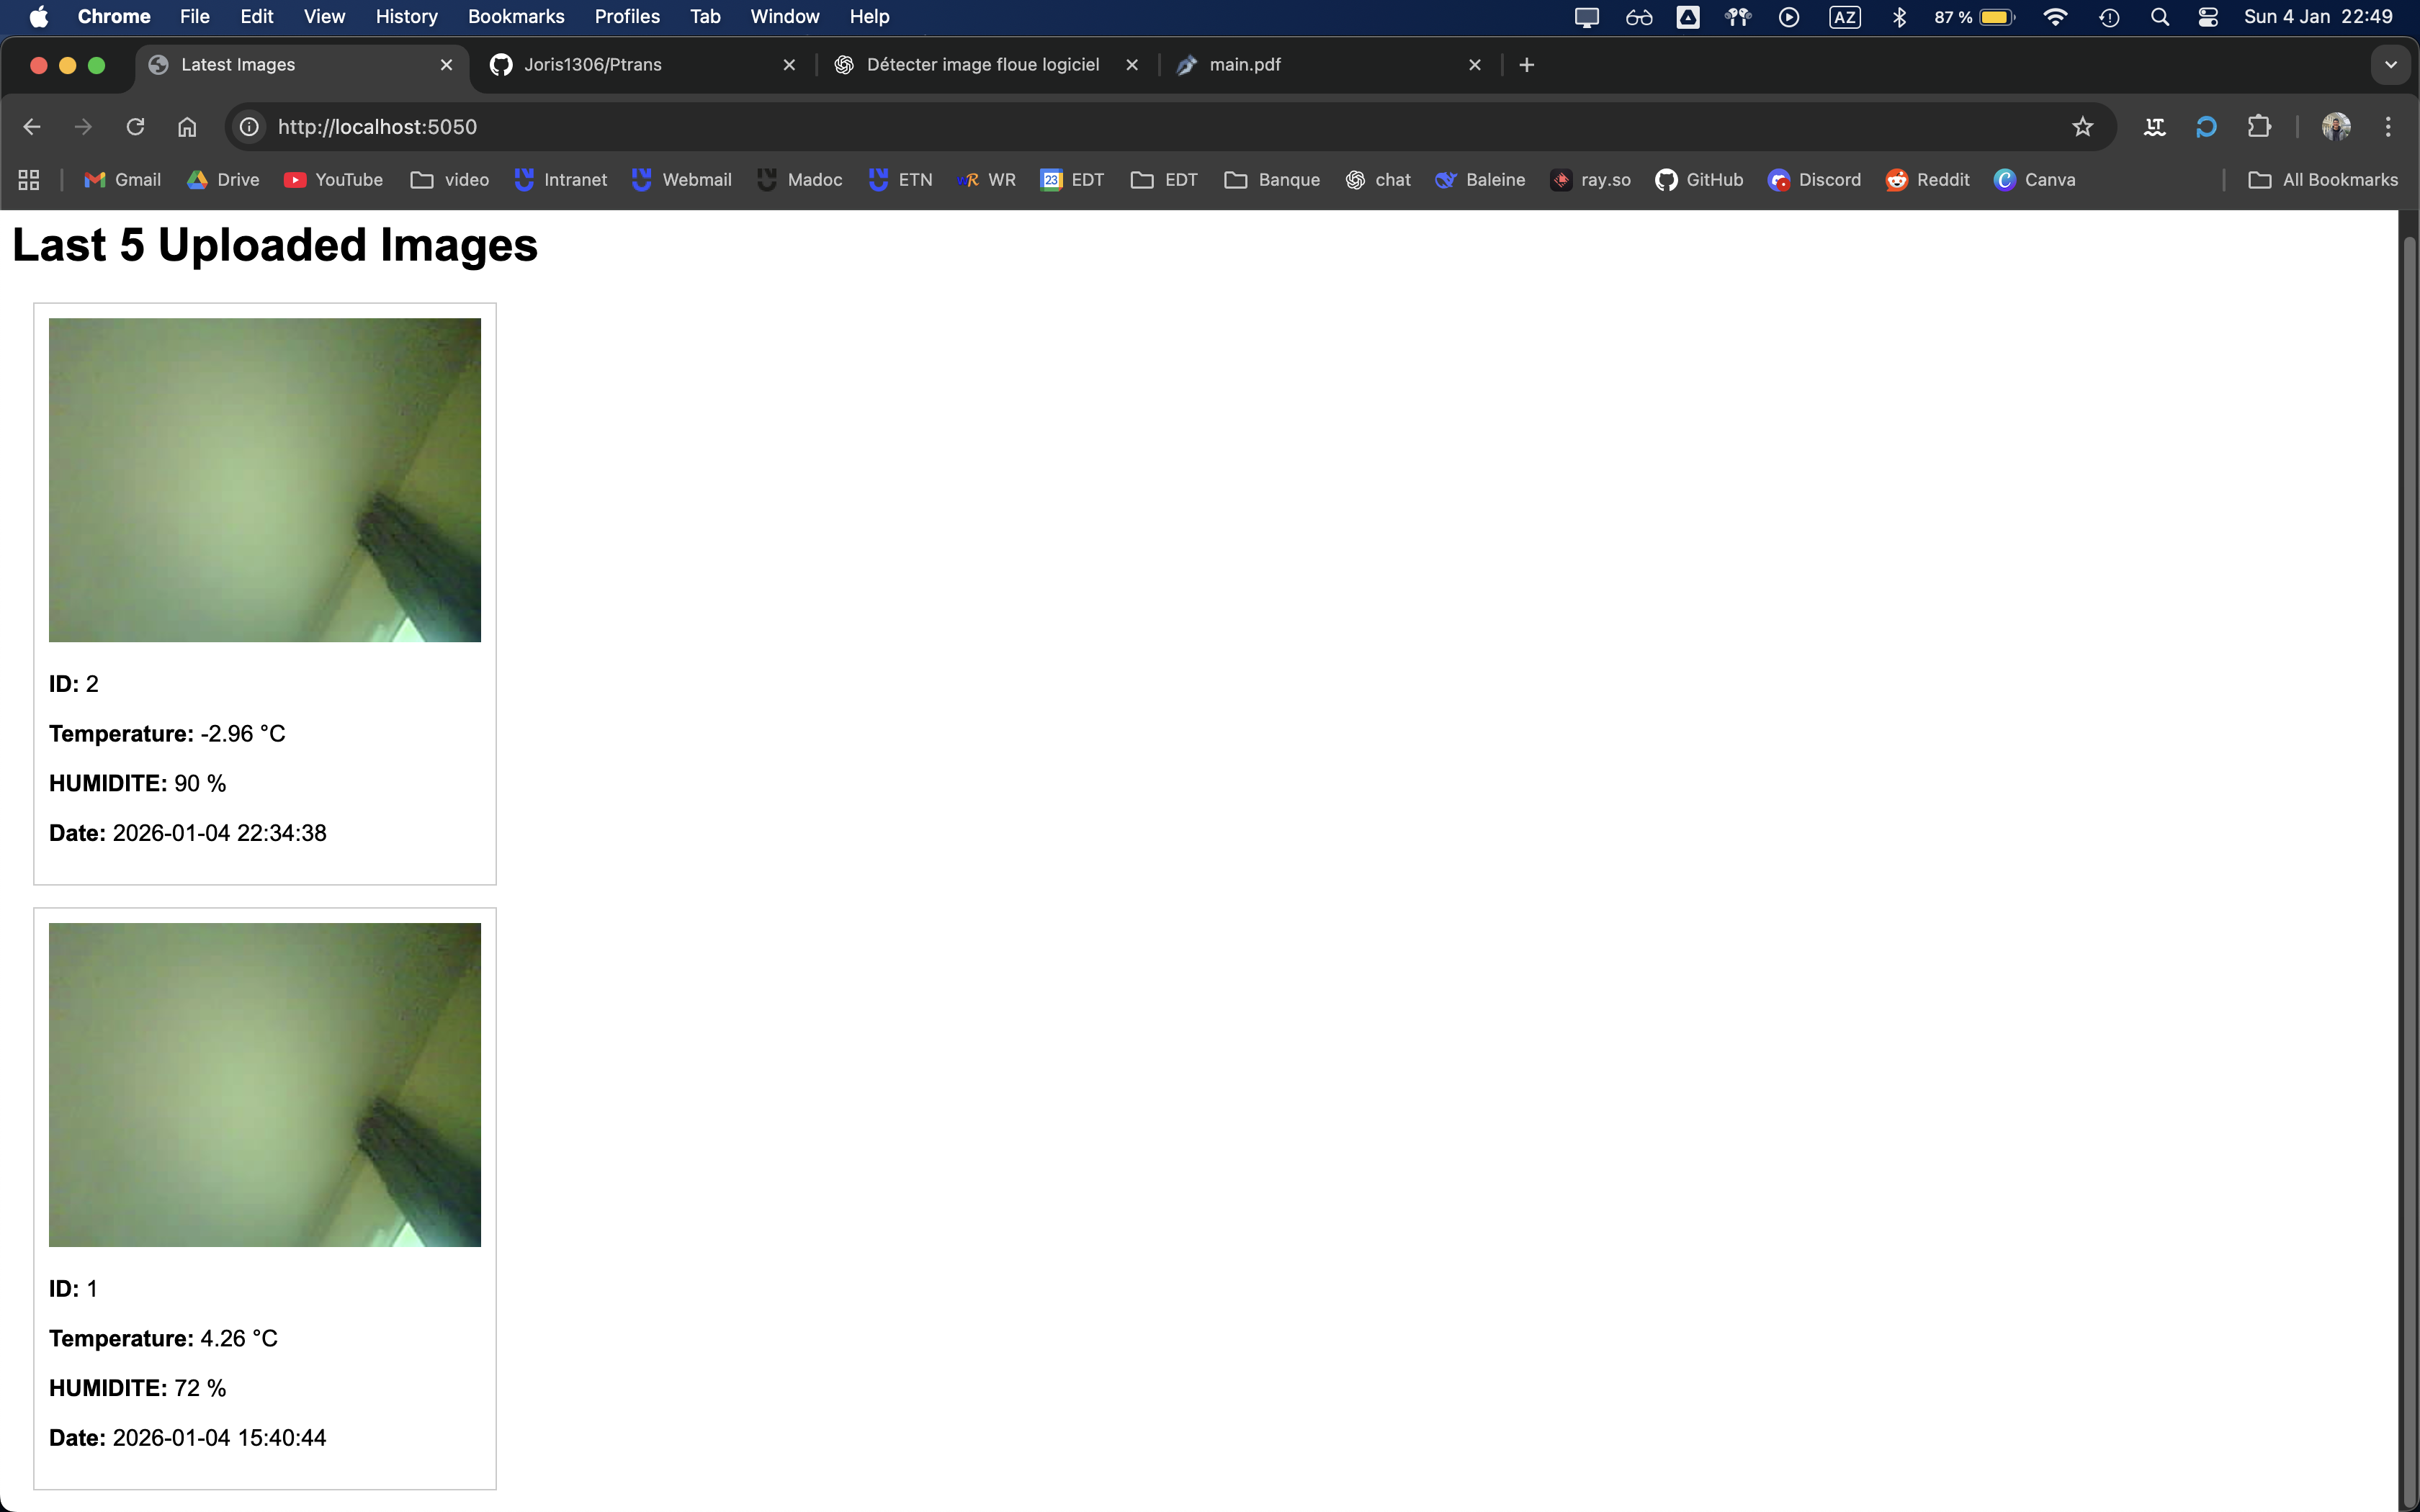
\includegraphics[width=0.8\textwidth]{include/sql_image/webpage.png}
    \caption{Affichage web simple des images stockées dans la base de données SQL}
    \label{fig:sql_web_view}
\end{figure}

\subsection{Remarques}
\begin{itemize}
  \item le WP IHM est lié direcetement au chapitre \ref{sec:sql_affichage}
  \item créer un nouveau point de sortie pour le WP AI CLASSIFICATION
\end{itemize}